\documentclass{beamer}

\usetheme{Antibes}
\useinnertheme{rounded}


\title{Graph Theory and Simulation}
\author{Matthew Hall}
\date{\today}

\begin{document}

\frame{\titlepage}

\section[Outline]{}
\frame{\tableofcontents}

\section{Graph Theory}


\subsection{Graphs}
\frame {
	\frametitle{Nodes and Edges}
	\begin{itemize}
		\item Nodes
		\item Edges
			\begin{itemize}
				\item Weights
				\item Direction
				\item Only need the immediate neighbors
			\end{itemize}
		\item http://compgeom.cs.uiuc.edu/~jeffe/teaching/algorithms/
		\item http://www.win.tue.nl/~nikhil/courses/2012/2WO08/max-flow-applications-4up.pdf
	\end{itemize}
}


\frame {
	\frametitle{Example}
	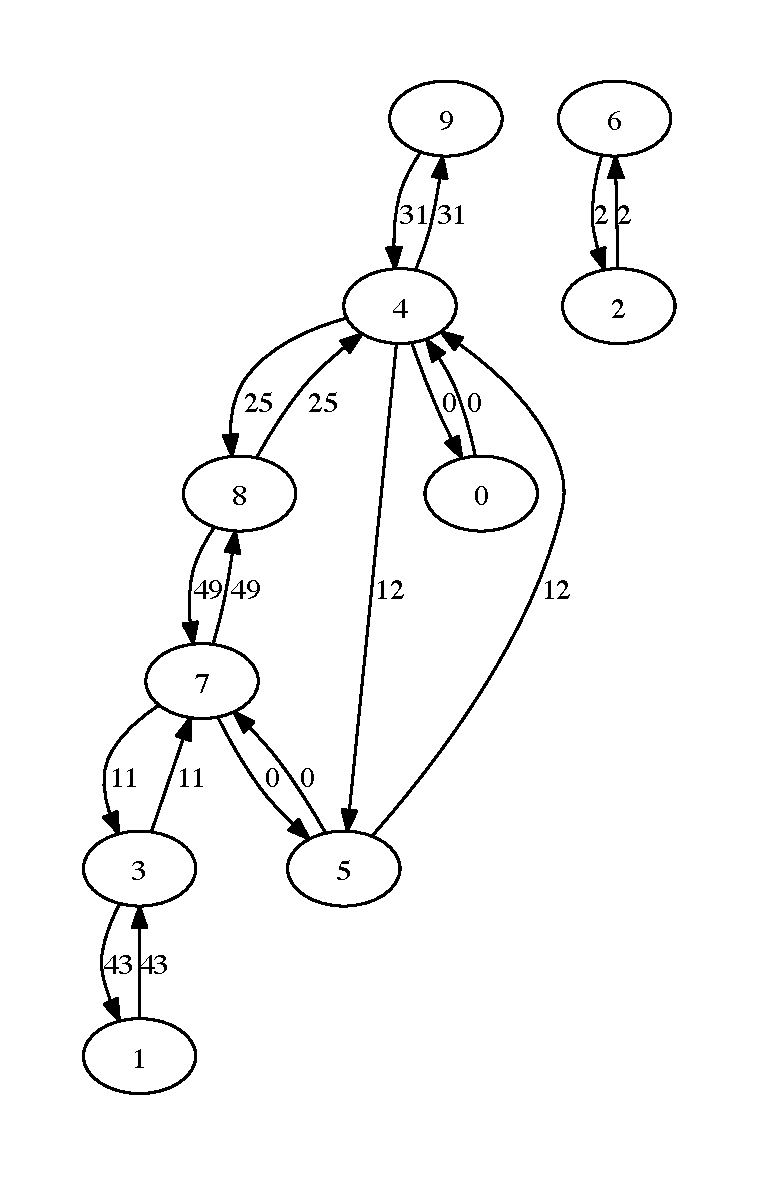
\includegraphics[width=2in]{talk.pdf}
}

\frame {
	\frametitle{Example}
	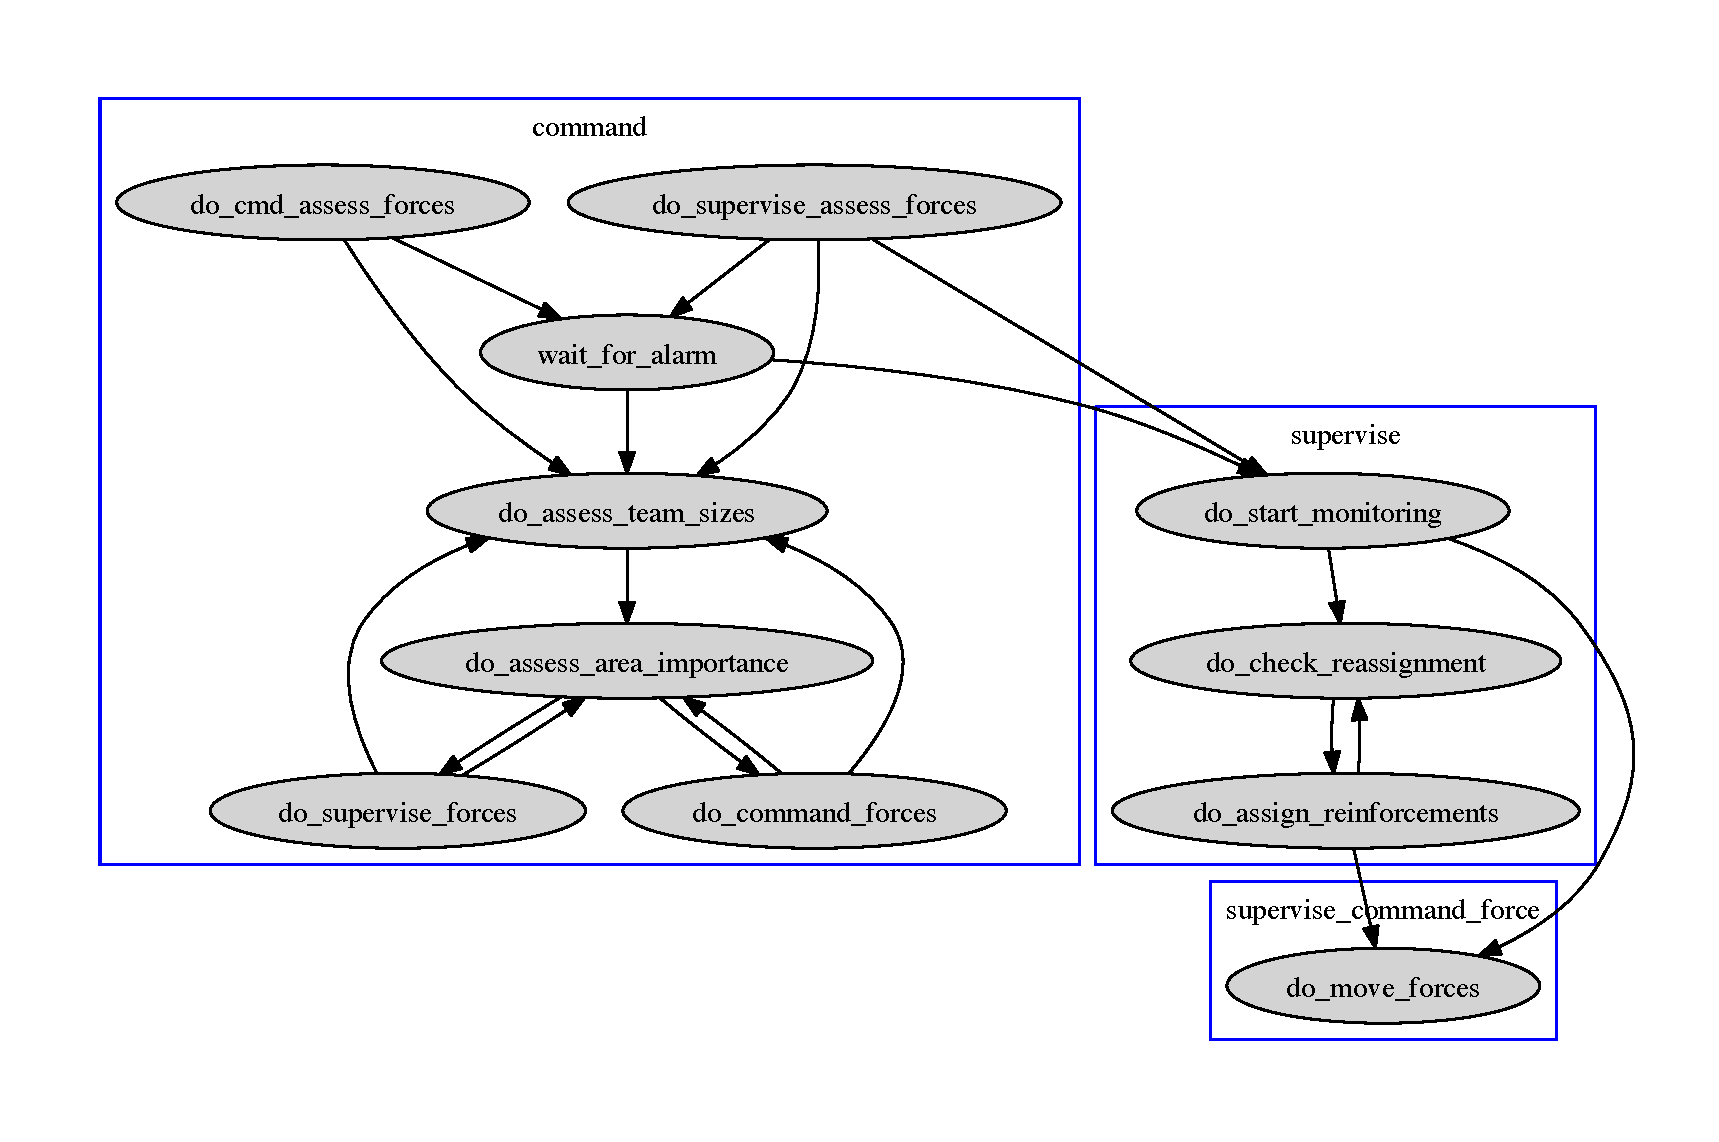
\includegraphics[width=3.8in]{command.pdf}
	\begin{itemize}
	  	\item Motivation: I have nodes and their list of neighbors, what can I do?
	\end{itemize}
}

\subsection{Types of Problems}
\frame {
	\frametitle{Data Representation}
	\begin{itemize}
		\item Draw communication networks
		\item Draw train of thought
		\item Interactions between players
	\end{itemize}
}

\frame {
	\frametitle{Algorithms}
	\begin{itemize}
		\item Visit Every Node (DFS, BFS)
		\item Shortest Path (A*)
		\item Spanning Tree
		\item Coloring
		\item Connected Components
		\item Social interaction mining (6 degrees of Kevin Bacon)
		\item ... Lots more to do ...
		\item Min Flow / Max Flow
	\end{itemize}
}

\section{Max Flow / Min Cut}
\subsection{Problem Setup}


\frame {
	\frametitle{Find the Maximum Flow}
	\begin{itemize}
		\item Source (s)
		\item Sink (t)
		\item Flow is conserved at each node
		\item Source Flow = Sink Flow
	\end{itemize}
}

\frame {
	\frametitle{Example Flow}
	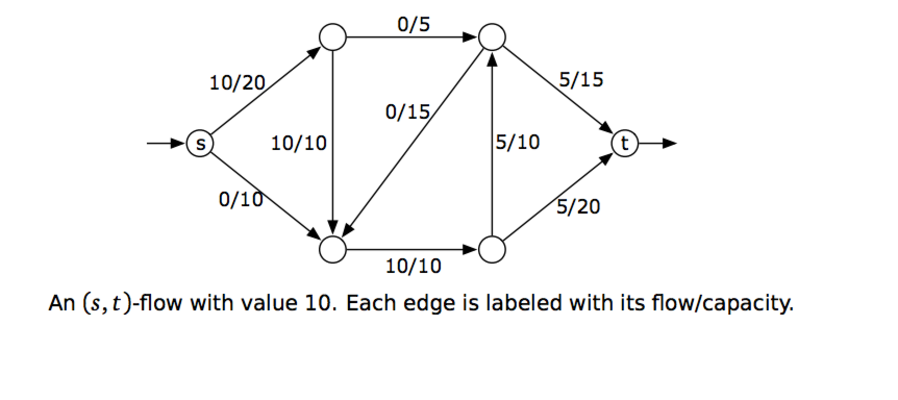
\includegraphics[width=4in]{flow.pdf}
}

\frame {
	\frametitle{Cuts}
	\begin{itemize}
		\item A cut is a separation of vertexes. For min flow, it is often called the (S,T) cut.
		\item The capacity of a cut is the sum of the capacities of the edges going from a vertex in S to a vertex in T.
		\item Maximum flow of a graph is equal to the minimum cut!
	\end{itemize}
}

\frame {
	\frametitle{Example Cut}
	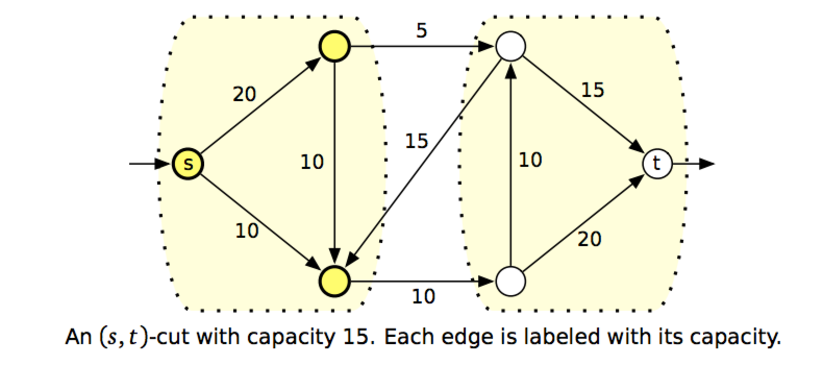
\includegraphics[width=4in]{cut.pdf}
}

\frame {
	\frametitle{Earliest Usage}
	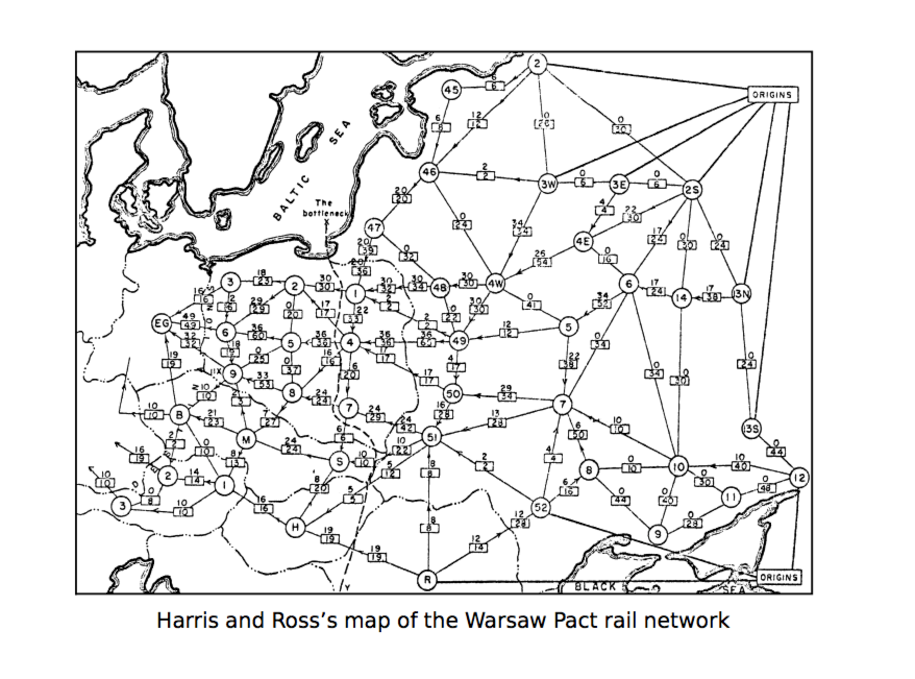
\includegraphics[width=4in]{warsaw.pdf}
}

\frame {
	\frametitle{Algorithms}
	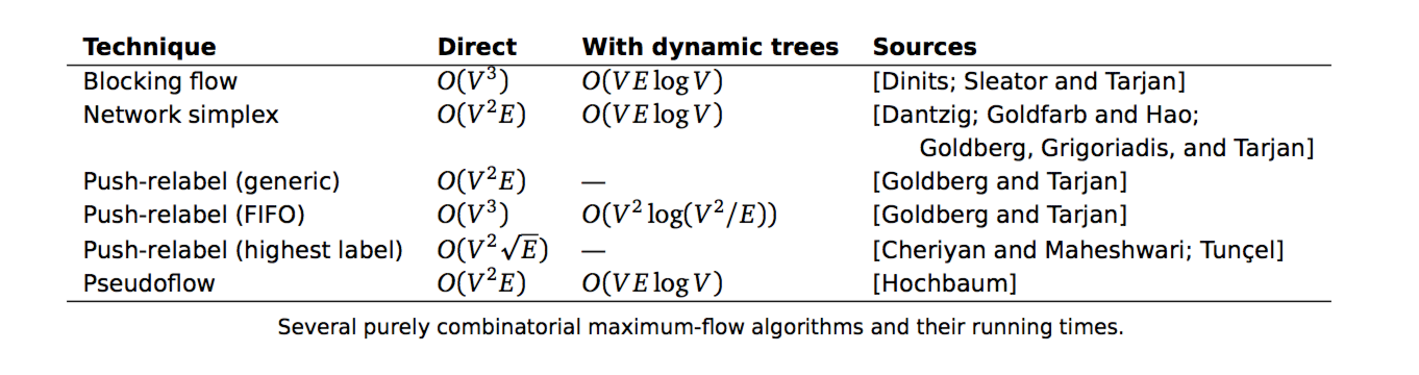
\includegraphics[width=5in]{algo.pdf}
	\begin{itemize}
		\item Take it on faith that this problem is solved efficiently
		\item Lots of approaches with reasonable running times
	\end{itemize}
}

\frame {
	\frametitle{What can we do?}
	\begin{itemize}
		\item Find maximum capacity of a network
		\item Find the bottleneck of a network
		\item Matching!
	\end{itemize}
}

\subsection{Bipartite}
\frame {
	\frametitle{What is it?}
In the mathematical field of graph theory, a bipartite graph (or bigraph) is a graph whose vertices can be divided into two disjoint sets  U and V  such that every edge connects a vertex in  U to one in V; that is,  and  are each independent sets. Equivalently, a bipartite graph is a graph that does not contain any odd-length cycles. (Wikipedia)
}


\frame {
	\frametitle{Example}
	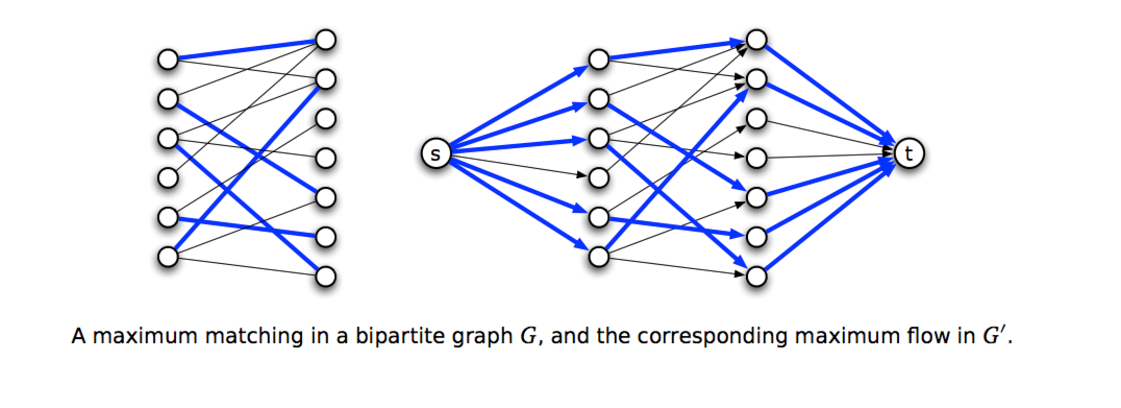
\includegraphics[width=4in]{bipartite.pdf}
}

\frame {
	\frametitle{So what?}
	\begin{itemize}
		\item We can convert matching problems into a bipartite graph and then find the maximum flow.
		\item And??????
		\item And, we can find the maximal or perfect match.
		\item And, by changing the way the graph is constructed, we can control the matching.
	\end{itemize}
}

\section{Example Uses}


\frame {
	\frametitle{Multiple Commodity}
	\begin{itemize}
		\item Run multiple types of commodities
		\item Must be fractional flows (integral flows is much harder)
	\end{itemize}
}

\frame {
	\frametitle{Multiple Tiers of Matching}
	\begin{itemize}
		\item Problem: Assign resources to multiple dependent targets
		\item Solution: Max flow with tiers connected from layer 1 to layer 2 to ...  layer n
	\end{itemize}
}

\frame {
	\frametitle{Separation of foreground and background in images}
	\begin{itemize}
		\item	Construct flow from source (foreground) to sink (background)
		\item Pixels are connected to minimize transition from foreground to background
		\item Extra terms to smooth the transition
	\end{itemize}
}

\frame {
	\frametitle{Separation of foreground and background in images}
	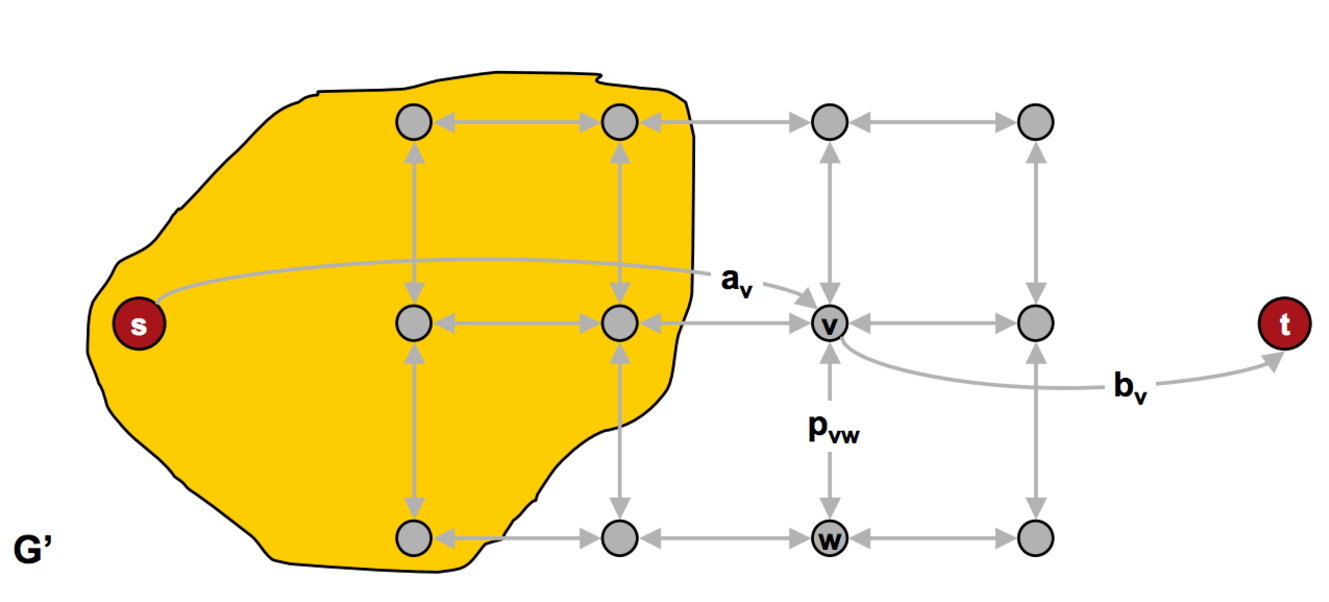
\includegraphics[width=4in]{image.pdf}
}

\section{Simulation Applications}
\subsection{Matching}
\frame {
	\frametitle{Matching Sniper Perches to Targets}
	\begin{itemize}
		\item Sniper Locations are S
		\item Targets Locations are T
		\item Maximal matching is each sniper having enough (or the most targets) and each
		target not having too much firepower assigned
		\item We can also assign weapons to each sniper
		\item What about too many targets to overwhelm the sniper???
		\item Can we represent movement????
	\end{itemize}
}

\frame {
	\frametitle{Matching Weapon Systems to Targets in React}
	\begin{itemize}
		\item Weapons are S
		\item Targets are T
		\item Maximal matching is each weapon having a target and no target is getting excessive firepower
		\item Is this reasonable for missile defense? people?
	\end{itemize}
}

\frame {
	\frametitle{Matching People to Coverspots}
	\begin{itemize}
		\item People are S
		\item Cover Locations are T
		\item Maximal matching is each person having cover and each
		person walking the shortest distance 
		\item We can also assign people based on the weapon they carry
		\item Is this reasonable for people to do? 
		\item Would they have planned this? 
		\item What about the defenders?
		\item What about supervisors?
	\end{itemize}
}

\frame {
	\frametitle{More Matching}
	\begin{itemize}
		\item People to patrol zones
		\item Ambulances to hospitals
		\item Teachers to students to classrooms
	\end{itemize}
}

\subsection{Flow}
\frame {
	\frametitle{Traffic Flow}
	\begin{itemize}
		\item Pipes, cars, rivers, trains, etc
		\item Traffic disruption
		\begin{itemize}
			\item Attack teleco
			\item Attack shipping
			\item Attack any linear infrastructure
		\end{itemize}
	\end{itemize}
}

\frame {
	\frametitle{Safety / Risk}
	\begin{itemize}
		\item Edge weights are probability of failure or success
		\item The bottleneck is where the risk is highest
		\item If I pass this threshold, its smooth sailing.
		\item If I improve the cut, I have an overall safer system.
		\item Shortest path is also really useful in this case!
	\end{itemize}
}


\section{Vertex Cover}
\frame {
	\frametitle{Definition}
	\begin{itemize}
	 	\item a vertex cover of a graph is a set of vertices such that each edge of the graph is incident to at least one vertex of the set.
		\item Minimum vertex cover is NP-Hard
	\end{itemize}
}

\frame {
	\frametitle{Approximation}
	\begin{itemize}
	 	\item Getting a vertex cover within 2n of real cover can be done in polynomial time
	\end{itemize}
}

\section{Conclusion}
\frame {
	\frametitle{Conclusion}
	\begin{block}{Graphs}
		\begin{itemize}
		\item Lots of  algorithms
		\item Easy to implement
		\item Lots of uses
		\end{itemize}
	\end{block}
	
	\begin{block}
		{Resources}
		\begin{itemize}
			\item Boost Graph Library (BGL)
			\item The Big Book of Algorithms
		\end{itemize}
	\end{block}
}


\end{document}
